\documentclass[12pt,a4paper]{article}
\usepackage{amsmath, amssymb, geometry, booktabs, xcolor, hyperref,
            listings, pgfplots, tcolorbox, enumitem, fancyhdr, tikz, array}
\usepgfplotslibrary{fillbetween}
\geometry{margin=2.5cm}
\pgfplotsset{compat=1.18}
\tcbuselibrary{skins, breakable}

\newtcolorbox{curiositybox}[1]{colback=yellow!10, colframe=orange!80, title=#1, breakable}
\newtcolorbox{infobox}[1]{colback=blue!5, colframe=blue!60, title=#1, breakable}
\newtcolorbox{mistakebox}[1]{colback=red!5, colframe=red!60, title=#1, breakable}
\newtcolorbox{learnbox}[1]{colback=green!5, colframe=green!60, title=#1, breakable}

\pagestyle{fancy}
\fancyhf{}
\lhead{Iterative Methods}
\rhead{Unit 1 --- LAC}
\cfoot{\thepage}

\title{\textbf{Iterative Methods: Jacobi Method and Gauss-Seidel Method} \\
       \large Unit 1 --- Matrix Algebra and Linear Systems}
\author{Department of Mathematics}
\date{\today}

\begin{document}
\maketitle
\tableofcontents
\newpage

%=====================================================================
\section{Real-World Engineering Hook}
%=====================================================================

\begin{curiositybox}{How Does a Power Grid Stay Balanced? Iterative Methods at Work}
Consider the IEEE 118-bus power system---a benchmark network with 118 buses, 54 generators,
and 186 transmission lines. Every second, power system engineers must solve a \textbf{load flow}
(power flow) problem: given the power injections at each bus, find the voltage magnitude and
phase angle at every node. This problem reduces to solving a large system of nonlinear equations
whose linearised form is a \(118 \times 118\) (or larger) sparse linear system.

Direct methods such as Gaussian elimination would fill in the sparse structure, dramatically
increasing memory and computation. Instead, power engineers use the \textbf{Gauss-Seidel}
load flow method: start from a ``flat start'' (all voltages \(= 1\angle 0^{\circ}\)), then update
each bus voltage one at a time using the most recently computed neighbour values. Within 20--50
iterations, the solution converges to the actual operating voltages with millivolt accuracy.

Beyond power systems, iterative methods drive:
\begin{itemize}
  \item \textbf{Heat conduction FD solvers} --- temperature distribution in turbine blades
  \item \textbf{Structural FEA} --- displacement fields in large truss/frame structures
  \item \textbf{Google PageRank} --- iterative eigenvector computation on a billion-node graph
\end{itemize}
Every time you load a webpage, stream a video, or fly in an aircraft, iterative linear solvers
are working behind the scenes. This lecture hands you the keys to understanding them from scratch.
\end{curiositybox}

%=====================================================================
\section{Why This Topic Exists}
%=====================================================================

\begin{center}
\begin{tabular}{@{}llll@{}}
\toprule
\textbf{Sub-Topic} & \textbf{Engineering Consequence} & \textbf{Why Critical} & \textbf{Scale} \\
\midrule
Diagonal Dominance &
  Guarantees convergence of iterative solver &
  Without it, solver may diverge &
  Precondition check \\
\addlinespace
Jacobi Method &
  Parallel voltage update in power networks &
  All old values used simultaneously &
  \(10^3\)--\(10^6\) unknowns \\
\addlinespace
Gauss-Seidel Method &
  Fast load-flow convergence in IEEE test cases &
  Immediate use of new values &
  \(\approx 2\times\) fewer iterations \\
\addlinespace
Convergence Analysis &
  Predicts solver success before running it &
  Spectral radius \(\rho(B)<1\) is the criterion &
  Design-time guarantee \\
\bottomrule
\end{tabular}
\end{center}

\begin{learnbox}{Why Engineers Must Master Iterative Methods}
Iterative methods are the engine of large-scale engineering simulation --- master them.
Direct solvers cost \(\mathcal{O}(n^3)\) operations; for a \(10^6 \times 10^6\) FEA system
that is \(10^{18}\) flops --- computationally impossible. Iterative methods cost
\(\mathcal{O}(kn)\) where \(k\) is the iteration count, typically a few dozen. This is
the difference between a simulation that runs in minutes and one that never finishes.
\end{learnbox}

%=====================================================================
\section{Intuition and Definitions}
%=====================================================================

\subsection{Diagonal Dominance --- Convergence Precondition}

Imagine you are trying to find the temperature at three points along a rod. Each equation
says: ``the temperature here is mostly determined by the heat source here, with small
corrections from the neighbours.'' If the self-influence (diagonal) dominates the
neighbour-influence (off-diagonal), the iterative correction process will tighten around
the true answer. If the neighbours dominate, corrections can overshoot and the iteration
spirals away. Diagonal dominance is the mathematical way to say ``self-influence wins.''

\begin{infobox}{Diagonal Dominance --- Formal Definition and Theorem}
\textbf{Definition.} An \(n \times n\) matrix \(A\) is \textbf{strictly diagonally dominant}
if for every row \(i\):
\[
  |a_{ii}| > \sum_{\substack{j=1\\j\neq i}}^{n} |a_{ij}| \qquad \text{for all } i = 1, 2, \ldots, n.
\]

\textbf{Row-wise check procedure:}
For each row \(i\), compute \(D_i = |a_{ii}|\) and \(S_i = \sum_{j \neq i}|a_{ij}|\).
The matrix is strictly diagonally dominant iff \(D_i > S_i\) for \emph{all} rows.

\textbf{Convergence Theorem.} If \(A\) is strictly diagonally dominant, then
both the Jacobi method and the Gauss-Seidel method converge for any initial guess
\(\mathbf{x}^{(0)}\).

\textbf{Rearrangement Strategy.} If the original system is not diagonally dominant,
permute the rows (and/or columns) so that the largest-magnitude element in each column
appears on the diagonal. Such a permutation always exists if the matrix is non-singular
(partial pivoting idea).
\end{infobox}

\textbf{Worked Example --- Diagonal Dominance Check}

Test the matrix from the system
\(4x_1 + x_2 - x_3 = 5\),\quad \(2x_1 + 7x_2 + x_3 = 19\),\quad \(x_1 - 3x_2 + 12x_3 = 22\).

\[
A = \begin{pmatrix} 4 & 1 & -1 \\ 2 & 7 & 1 \\ 1 & -3 & 12 \end{pmatrix}
\]

\begin{center}
\begin{tabular}{@{}ccccl@{}}
\toprule
Row \(i\) & \(|a_{ii}|\) & \(\sum_{j\neq i}|a_{ij}|\) & Condition & Verdict \\
\midrule
1 & \(|4|=4\)  & \(|1|+|-1|=2\)   & \(4>2\) & \checkmark\ Satisfied \\
2 & \(|7|=7\)  & \(|2|+|1|=3\)    & \(7>3\) & \checkmark\ Satisfied \\
3 & \(|12|=12\)& \(|1|+|-3|=4\)   & \(12>4\)& \checkmark\ Satisfied \\
\bottomrule
\end{tabular}
\end{center}

\textbf{Conclusion:} All three rows satisfy the diagonal dominance condition. Both
Jacobi and Gauss-Seidel are guaranteed to converge for this system.

\subsection{Jacobi Iteration Method}

Picture ten friends each trying to solve one equation for one unknown. Every friend
looks at \emph{yesterday's} guesses of all the others, computes their new answer,
and everyone reveals their new answer at the same moment --- like a simultaneous vote.
No one sees anyone else's new answer until the next round. This is the Jacobi method:
completely parallel, completely fair, but potentially slow because new information
propagates with a one-round delay.

\begin{infobox}{Jacobi Method --- Full Derivation and Formulae}
\textbf{Setup.} Solve \(A\mathbf{x} = \mathbf{b}\) where
\(A = \begin{pmatrix} a_{11} & \cdots & a_{1n} \\ \vdots & \ddots & \vdots \\
a_{n1} & \cdots & a_{nn}\end{pmatrix}\).

\textbf{Derivation.} From row \(i\):
\[
  a_{i1}x_1 + \cdots + a_{ii}x_i + \cdots + a_{in}x_n = b_i.
\]
Isolate \(x_i\):
\[
  x_i^{(k+1)} = \frac{1}{a_{ii}}\!\left[b_i - \sum_{\substack{j=1\\j\neq i}}^{n} a_{ij}\,x_j^{(k)}\right], \quad i = 1,\ldots,n.
\]
\textbf{Key rule:} ALL values on the right use iteration \(k\) (old values only).

\textbf{Matrix Splitting Form.} Split \(A = D + L + U\) where \(D\) is diagonal,
\(L\) is strictly lower triangular, \(U\) is strictly upper triangular. Then:
\[
  \mathbf{x}^{(k+1)} = D^{-1}\!\left(\mathbf{b} - (L+U)\mathbf{x}^{(k)}\right)
                       = \underbrace{-D^{-1}(L+U)}_{B_J}\mathbf{x}^{(k)} + D^{-1}\mathbf{b}.
\]
The Jacobi iteration matrix is \(B_J = -D^{-1}(L+U)\).

\textbf{Convergence Criterion.} Sufficient condition: strict diagonal dominance.
Necessary and sufficient: spectral radius \(\rho(B_J) < 1\).

\textbf{Stopping Criterion.}
\[
  \max_{i}\left|x_i^{(k+1)} - x_i^{(k)}\right| < \varepsilon,
\]
where \(\varepsilon\) is a user-specified tolerance (e.g.\ \(\varepsilon = 10^{-4}\)).
\end{infobox}

\textbf{Worked Example --- Jacobi Method (4 Iterations)}

Solve: \(4x_1 + x_2 - x_3 = 5\),\quad \(2x_1 + 7x_2 + x_3 = 19\),\quad
\(x_1 - 3x_2 + 12x_3 = 22\).\quad Start: \(\mathbf{x}^{(0)} = (0,0,0)^T\).

\textbf{Jacobi iteration formulas:}
\begin{align*}
x_1^{(k+1)} &= \tfrac{1}{4}\!\left[5 - x_2^{(k)} + x_3^{(k)}\right] \\
x_2^{(k+1)} &= \tfrac{1}{7}\!\left[19 - 2x_1^{(k)} - x_3^{(k)}\right] \\
x_3^{(k+1)} &= \tfrac{1}{12}\!\left[22 - x_1^{(k)} + 3x_2^{(k)}\right]
\end{align*}

\textbf{Iteration 1} (using \(x_1^{(0)}=0, x_2^{(0)}=0, x_3^{(0)}=0\)):
\begin{align*}
x_1^{(1)} &= \tfrac{1}{4}[5 - 0 + 0] = 1.2500 \\
x_2^{(1)} &= \tfrac{1}{7}[19 - 0 - 0] = 2.7143 \\
x_3^{(1)} &= \tfrac{1}{12}[22 - 0 + 0] = 1.8333
\end{align*}
Max error \(= \max(|1.2500|, |2.7143|, |1.8333|) = 2.7143\).

\textbf{Iteration 2} (using \(x_1^{(1)}=1.2500, x_2^{(1)}=2.7143, x_3^{(1)}=1.8333\)):
\begin{align*}
x_1^{(2)} &= \tfrac{1}{4}[5 - 2.7143 + 1.8333] = \tfrac{4.1190}{4} = 1.0298 \\
x_2^{(2)} &= \tfrac{1}{7}[19 - 2(1.2500) - 1.8333] = \tfrac{14.6667}{7} = 2.0952 \\
x_3^{(2)} &= \tfrac{1}{12}[22 - 1.2500 + 3(2.7143)] = \tfrac{28.8929}{12} = 2.4077
\end{align*}
Max error \(= \max(|1.0298-1.2500|, |2.0952-2.7143|, |2.4077-1.8333|)
= \max(0.2202, 0.6191, 0.5744) = 0.6191\).

\textbf{Iteration 3} (using \(x_1^{(2)}=1.0298, x_2^{(2)}=2.0952, x_3^{(2)}=2.4077\)):
\begin{align*}
x_1^{(3)} &= \tfrac{1}{4}[5 - 2.0952 + 2.4077] = \tfrac{5.3125}{4} = 1.3281 \\
x_2^{(3)} &= \tfrac{1}{7}[19 - 2(1.0298) - 2.4077] = \tfrac{14.5327}{7} = 2.0761 \\
x_3^{(3)} &= \tfrac{1}{12}[22 - 1.0298 + 3(2.0952)] = \tfrac{27.2558}{12} = 2.2713
\end{align*}
Max error \(= \max(|1.3281-1.0298|,|2.0761-2.0952|,|2.2713-2.4077|)
= \max(0.2983, 0.0191, 0.1364) = 0.2983\).

\textbf{Iteration 4} (using \(x_1^{(3)}=1.3281, x_2^{(3)}=2.0761, x_3^{(3)}=2.2713\)):
\begin{align*}
x_1^{(4)} &= \tfrac{1}{4}[5 - 2.0761 + 2.2713] = \tfrac{5.1952}{4} = 1.2988 \\
x_2^{(4)} &= \tfrac{1}{7}[19 - 2(1.3281) - 2.2713] = \tfrac{14.0725}{7} = 2.0104 \\
x_3^{(4)} &= \tfrac{1}{12}[22 - 1.3281 + 3(2.0761)] = \tfrac{26.8997}{12} = 2.2416
\end{align*}
Max error \(= \max(|1.2988-1.3281|,|2.0104-2.0761|,|2.2416-2.2713|)
= \max(0.0293, 0.0657, 0.0297) = 0.0657\).

\textbf{Full Jacobi Iteration Table:}

\begin{center}
\begin{tabular}{@{}ccccc@{}}
\toprule
Iteration \(k\) & \(x_1^{(k)}\) & \(x_2^{(k)}\) & \(x_3^{(k)}\) & Max Error \\
\midrule
0 & 0.0000 & 0.0000 & 0.0000 & --- \\
1 & 1.2500 & 2.7143 & 1.8333 & 2.7143 \\
2 & 1.0298 & 2.0952 & 2.4077 & 0.6191 \\
3 & 1.3281 & 2.0761 & 2.2713 & 0.2983 \\
4 & 1.2988 & 2.0104 & 2.2416 & 0.0657 \\
Exact & 1.3000 & 2.0000 & 2.2500 & --- \\
\bottomrule
\end{tabular}
\end{center}

\textit{Exact solution} (by substitution): \(x_1=1.3,\; x_2=2.0,\; x_3=2.25\).
After 4 iterations, Jacobi is within \(\approx 0.07\) of the exact solution.

\subsection{Gauss-Seidel Iteration Method}

Now picture the same ten friends, but this time whenever someone computes a new answer,
they immediately whisper it to the friends who haven't computed theirs yet. Each person
uses the \emph{freshest} available information. This is Gauss-Seidel: sequential, slightly
less parallel, but information propagates within the same round, so convergence is faster.
The mathematical guarantee is the same (diagonal dominance suffices), but roughly twice
as many Jacobi steps are needed to match one round of Gauss-Seidel's accuracy.

\begin{infobox}{Gauss-Seidel Method --- Full Derivation and Formulae}
\textbf{Derivation.} From row \(i\), isolate \(x_i\) but now use already-updated
values \(x_j^{(k+1)}\) for \(j < i\) and old values \(x_j^{(k)}\) for \(j > i\):
\[
  x_i^{(k+1)} = \frac{1}{a_{ii}}\!\left[
    b_i - \sum_{j=1}^{i-1} a_{ij}\,x_j^{(k+1)} - \sum_{j=i+1}^{n} a_{ij}\,x_j^{(k)}
  \right], \quad i = 1,\ldots,n.
\]
\textbf{Key rule:} Uses the newest available value for each variable --- sequential update.

\textbf{Matrix Splitting Form.}
\[
  (D+L)\mathbf{x}^{(k+1)} = \mathbf{b} - U\mathbf{x}^{(k)},
\]
\[
  \mathbf{x}^{(k+1)} = \underbrace{-(D+L)^{-1}U}_{B_{GS}}\mathbf{x}^{(k)} + (D+L)^{-1}\mathbf{b}.
\]
The Gauss-Seidel iteration matrix is \(B_{GS} = -(D+L)^{-1}U\).

\textbf{Convergence.}
\begin{itemize}
  \item Sufficient: \(A\) strictly diagonally dominant (same condition as Jacobi).
  \item Necessary and sufficient: \(\rho(B_{GS}) < 1\).
  \item For symmetric positive definite \(A\): Gauss-Seidel always converges.
  \item Typical behaviour: \(\rho(B_{GS}) \approx \rho(B_J)^2\), meaning Gauss-Seidel
        needs roughly half as many iterations as Jacobi for the same accuracy.
\end{itemize}

\textbf{Stopping Criterion.} Same as Jacobi:
\[
  \max_{i}\left|x_i^{(k+1)} - x_i^{(k)}\right| < \varepsilon.
\]
\end{infobox}

\textbf{Worked Example --- Gauss-Seidel Method (4 Iterations) with Jacobi Comparison}

Same system: \(4x_1+x_2-x_3=5\), \(2x_1+7x_2+x_3=19\), \(x_1-3x_2+12x_3=22\).
Start: \(\mathbf{x}^{(0)}=(0,0,0)^T\).

\textbf{Gauss-Seidel formulas (sequential):}
\begin{align*}
x_1^{(k+1)} &= \tfrac{1}{4}\!\left[5 - x_2^{(k)} + x_3^{(k)}\right] \\
x_2^{(k+1)} &= \tfrac{1}{7}\!\left[19 - 2x_1^{(k+1)} - x_3^{(k)}\right]
  \quad\leftarrow\text{uses NEW }x_1^{(k+1)}\\
x_3^{(k+1)} &= \tfrac{1}{12}\!\left[22 - x_1^{(k+1)} + 3x_2^{(k+1)}\right]
  \quad\leftarrow\text{uses NEW }x_1^{(k+1)},\,x_2^{(k+1)}
\end{align*}

\textbf{Iteration 1} (from \((0,0,0)\)):
\begin{align*}
x_1^{(1)} &= \tfrac{1}{4}[5 - 0 + 0] = 1.2500 \\
x_2^{(1)} &= \tfrac{1}{7}[19 - 2(1.2500) - 0] = \tfrac{16.5000}{7} = 2.3571 \\
x_3^{(1)} &= \tfrac{1}{12}[22 - 1.2500 + 3(2.3571)] = \tfrac{27.8213}{12} = 2.3184
\end{align*}
Max error \(= \max(1.2500, 2.3571, 2.3184) = 2.3571\).

\textbf{Iteration 2} (from \((1.2500, 2.3571, 2.3184)\)):
\begin{align*}
x_1^{(2)} &= \tfrac{1}{4}[5 - 2.3571 + 2.3184] = \tfrac{4.9613}{4} = 1.2403 \\
x_2^{(2)} &= \tfrac{1}{7}[19 - 2(1.2403) - 2.3184] = \tfrac{14.2010}{7} = 2.0287 \\
x_3^{(2)} &= \tfrac{1}{12}[22 - 1.2403 + 3(2.0287)] = \tfrac{26.8458}{12} = 2.2372
\end{align*}
Max error \(= \max(|1.2403-1.2500|,|2.0287-2.3571|,|2.2372-2.3184|)
= \max(0.0097, 0.3284, 0.0812) = 0.3284\).

\textbf{Iteration 3} (from \((1.2403, 2.0287, 2.2372)\)):
\begin{align*}
x_1^{(3)} &= \tfrac{1}{4}[5 - 2.0287 + 2.2372] = \tfrac{5.2085}{4} = 1.3021 \\
x_2^{(3)} &= \tfrac{1}{7}[19 - 2(1.3021) - 2.2372] = \tfrac{14.1586}{7} = 2.0227 \\
x_3^{(3)} &= \tfrac{1}{12}[22 - 1.3021 + 3(2.0227)] = \tfrac{26.7660}{12} = 2.2305
\end{align*}
Max error \(= \max(|1.3021-1.2403|,|2.0227-2.0287|,|2.2305-2.2372|)
= \max(0.0618, 0.0060, 0.0067) = 0.0618\).

\textbf{Iteration 4} (from \((1.3021, 2.0227, 2.2305)\)):
\begin{align*}
x_1^{(4)} &= \tfrac{1}{4}[5 - 2.0227 + 2.2305] = \tfrac{5.2078}{4} = 1.3020 \\
x_2^{(4)} &= \tfrac{1}{7}[19 - 2(1.3020) - 2.2305] = \tfrac{14.1655}{7} = 2.0236 \\
x_3^{(4)} &= \tfrac{1}{12}[22 - 1.3020 + 3(2.0236)] = \tfrac{26.7688}{12} = 2.2307
\end{align*}
Max error \(= \max(|1.3020-1.3021|,|2.0236-2.0227|,|2.2307-2.2305|)
= \max(0.0001, 0.0009, 0.0002) = 0.0009\).

\textbf{Side-by-Side Comparison Table: Jacobi vs.\ Gauss-Seidel}

\begin{center}
\begin{tabular}{@{}c ccc ccc c@{}}
\toprule
& \multicolumn{3}{c}{\textbf{Jacobi}} & \multicolumn{3}{c}{\textbf{Gauss-Seidel}} & \\
\cmidrule(lr){2-4}\cmidrule(lr){5-7}
\(k\) & \(x_1\) & \(x_2\) & \(x_3\) & \(x_1\) & \(x_2\) & \(x_3\) & Max Err (GS) \\
\midrule
0 & 0.0000 & 0.0000 & 0.0000 & 0.0000 & 0.0000 & 0.0000 & --- \\
1 & 1.2500 & 2.7143 & 1.8333 & 1.2500 & 2.3571 & 2.3184 & 2.3571 \\
2 & 1.0298 & 2.0952 & 2.4077 & 1.2403 & 2.0287 & 2.2372 & 0.3284 \\
3 & 1.3281 & 2.0761 & 2.2713 & 1.3021 & 2.0227 & 2.2305 & 0.0618 \\
4 & 1.2988 & 2.0104 & 2.2416 & 1.3020 & 2.0236 & 2.2307 & 0.0009 \\
Exact & 1.3000 & 2.0000 & 2.2500 & 1.3000 & 2.0000 & 2.2500 & 0 \\
\bottomrule
\end{tabular}
\end{center}

\textit{Observation:} After 4 iterations, Gauss-Seidel achieves max error \(0.0009\)
versus Jacobi's \(0.0657\) --- roughly \(73\times\) smaller error in the same number of steps.

\subsection{Convergence Analysis and Matrix Splitting}

How do we know \emph{before} running an iteration whether it will converge?
The answer lies in the eigenvalues of the iteration matrix. Think of each iteration as
multiplying the error vector by \(B\): after \(k\) steps the error is multiplied by \(B^k\).
If all eigenvalues of \(B\) lie strictly inside the unit circle in the complex plane,
the error shrinks to zero. The largest eigenvalue magnitude --- the spectral radius ---
controls the convergence speed. A smaller spectral radius means faster convergence.

\begin{infobox}{Convergence Analysis --- Spectral Radius and Matrix Splitting}
\textbf{Matrix Splitting.} Write \(A = M - N\) so that \(Mx = Nx + b\) leads to
the iteration \(\mathbf{x}^{(k+1)} = M^{-1}N\mathbf{x}^{(k)} + M^{-1}\mathbf{b}\).

\begin{center}
\begin{tabular}{@{}lll@{}}
\toprule
Method & \(M\) & \(N\) \\
\midrule
Jacobi & \(D\) & \(-(L+U)\) \\
Gauss-Seidel & \(D+L\) & \(-U\) \\
\bottomrule
\end{tabular}
\end{center}

\textbf{Iteration matrices:}
\begin{align*}
B_J &= D^{-1}(L+U) \quad\text{(Jacobi)} \\
B_{GS} &= (D+L)^{-1}U \quad\text{(Gauss-Seidel)}
\end{align*}

\textbf{Spectral Radius.}
\[
  \rho(B) = \max_{i}|\lambda_i(B)|,
\]
where \(\lambda_i(B)\) are the eigenvalues of \(B\).

\textbf{Convergence Theorem (Necessary and Sufficient).}
The iteration \(\mathbf{x}^{(k+1)} = B\mathbf{x}^{(k)} + \mathbf{c}\) converges
for every starting point \(\mathbf{x}^{(0)}\) if and only if \(\rho(B) < 1\).

\textbf{Error reduction.} After \(k\) iterations:
\[
  \|\mathbf{e}^{(k)}\| \leq \|B\|^k \|\mathbf{e}^{(0)}\| \approx \rho(B)^k \|\mathbf{e}^{(0)}\|.
\]
A smaller \(\rho(B)\) gives faster convergence.

\textbf{Relationship between Jacobi and GS spectral radii.}
For consistently ordered matrices (e.g.\ tridiagonal):
\[
  \rho(B_{GS}) = \rho(B_J)^2.
\]
Hence Gauss-Seidel converges in approximately half as many iterations as Jacobi.
\end{infobox}

\textbf{Worked Example --- Spectral Radius Computation for a \(2 \times 2\) System}

Consider the \(2 \times 2\) system:
\[
A = \begin{pmatrix} 4 & 1 \\ 2 & 3 \end{pmatrix}, \quad
\mathbf{b} = \begin{pmatrix} 9 \\ 8 \end{pmatrix}.
\]
Split: \(D = \begin{pmatrix} 4 & 0 \\ 0 & 3 \end{pmatrix}\),
\(L = \begin{pmatrix} 0 & 0 \\ 2 & 0 \end{pmatrix}\),
\(U = \begin{pmatrix} 0 & 1 \\ 0 & 0 \end{pmatrix}\).

\textbf{Jacobi iteration matrix:}
\[
B_J = -D^{-1}(L+U)
= -\begin{pmatrix}1/4 & 0 \\ 0 & 1/3\end{pmatrix}
  \begin{pmatrix}0 & 1 \\ 2 & 0\end{pmatrix}
= \begin{pmatrix}0 & -1/4 \\ -2/3 & 0\end{pmatrix}.
\]
Characteristic equation: \(\det(B_J - \lambda I)=0\):
\[
  \lambda^2 - \frac{1}{4}\cdot\frac{2}{3} = 0 \implies \lambda^2 = \frac{1}{6}
  \implies \lambda = \pm\frac{1}{\sqrt{6}} \approx \pm 0.4082.
\]
So \(\rho(B_J) = \dfrac{1}{\sqrt{6}} \approx 0.4082 < 1\). Jacobi converges.

\textbf{Gauss-Seidel iteration matrix:}
\[
B_{GS} = -(D+L)^{-1}U
= -\begin{pmatrix}4 & 0 \\ 2 & 3\end{pmatrix}^{-1}\begin{pmatrix}0 & 1 \\ 0 & 0\end{pmatrix}.
\]
Compute \((D+L)^{-1} = \dfrac{1}{12}\begin{pmatrix}3 & 0 \\ -2 & 4\end{pmatrix}\):
\[
B_{GS} = -\frac{1}{12}\begin{pmatrix}3 & 0 \\ -2 & 4\end{pmatrix}
\begin{pmatrix}0 & 1 \\ 0 & 0\end{pmatrix}
= -\frac{1}{12}\begin{pmatrix}0 & 3 \\ 0 & -2\end{pmatrix}
= \begin{pmatrix}0 & -1/4 \\ 0 & 1/6\end{pmatrix}.
\]
Eigenvalues: \(\lambda = 0\) and \(\lambda = 1/6 \approx 0.1667\).
So \(\rho(B_{GS}) = \dfrac{1}{6} \approx 0.1667 < 1\). Gauss-Seidel converges.

\textbf{Comparison:}
\[
\rho(B_{GS}) = \frac{1}{6} \approx \left(\frac{1}{\sqrt{6}}\right)^2 = \rho(B_J)^2.
\]
This confirms the theoretical result: Gauss-Seidel converges roughly twice as fast as Jacobi
for this system.

%=====================================================================
\section{Visual Artifacts}
%=====================================================================

\subsection*{Visual 1: Convergence of \(x_1\) --- Jacobi vs.\ Gauss-Seidel}

\begin{center}
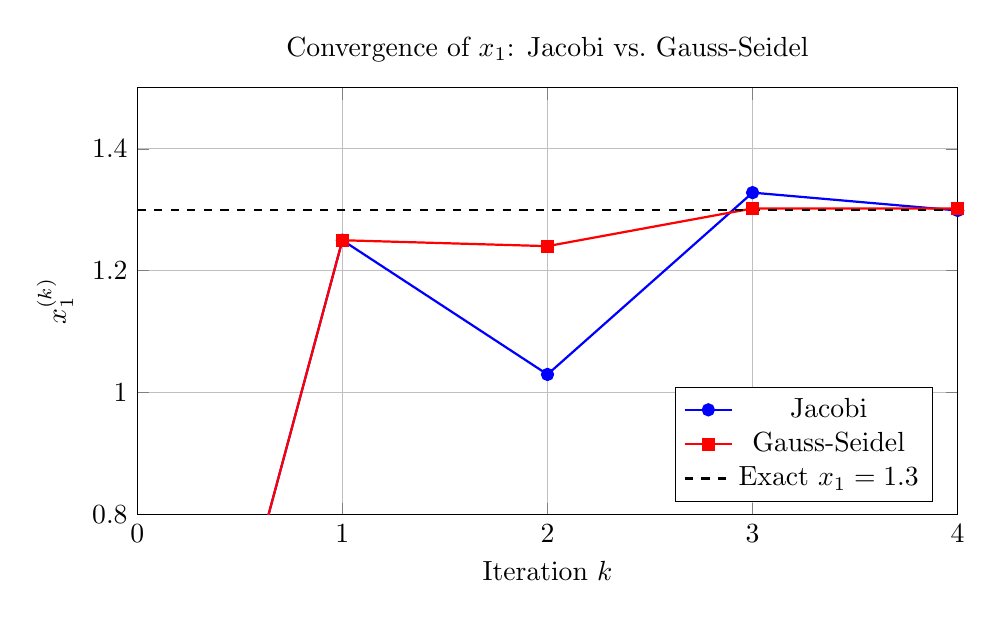
\begin{tikzpicture}
\begin{axis}[
  width=12cm, height=7cm,
  xlabel={Iteration \(k\)},
  ylabel={\(x_1^{(k)}\)},
  title={Convergence of \(x_1\): Jacobi vs.\ Gauss-Seidel},
  grid=both,
  legend pos=south east,
  xmin=0, xmax=4,
  ymin=0.8, ymax=1.5,
  xtick={0,1,2,3,4},
]
\addplot[blue, thick, mark=*] coordinates {
  (0,0.0000)(1,1.2500)(2,1.0298)(3,1.3281)(4,1.2988)
};
\addlegendentry{Jacobi}
\addplot[red, thick, mark=square*] coordinates {
  (0,0.0000)(1,1.2500)(2,1.2403)(3,1.3021)(4,1.3020)
};
\addlegendentry{Gauss-Seidel}
\addplot[black, dashed, thick] coordinates {(0,1.3)(4,1.3)};
\addlegendentry{Exact \(x_1=1.3\)}
\end{axis}
\end{tikzpicture}
\end{center}

\subsection*{Visual 2: Update Dependency Diagram}

\begin{center}
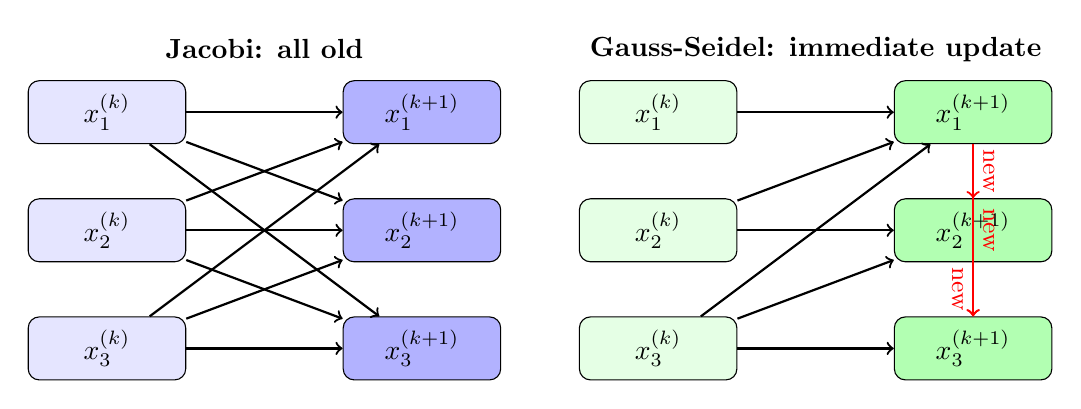
\begin{tikzpicture}[
  node distance=2.2cm,
  box/.style={draw, rounded corners, minimum width=2cm, minimum height=0.8cm, align=center},
  arrow/.style={->, thick},
  newarrow/.style={->, thick, red}
]
% Jacobi side
\node[box, fill=blue!10] (jx1old) at (0,3) {\(x_1^{(k)}\)};
\node[box, fill=blue!10] (jx2old) at (0,1.5) {\(x_2^{(k)}\)};
\node[box, fill=blue!10] (jx3old) at (0,0) {\(x_3^{(k)}\)};
\node[box, fill=blue!30] (jx1new) at (4,3) {\(x_1^{(k+1)}\)};
\node[box, fill=blue!30] (jx2new) at (4,1.5) {\(x_2^{(k+1)}\)};
\node[box, fill=blue!30] (jx3new) at (4,0) {\(x_3^{(k+1)}\)};
\node at (2,3.8) {\textbf{Jacobi: all old}};
\draw[arrow] (jx1old) -- (jx1new);
\draw[arrow] (jx2old) -- (jx1new);
\draw[arrow] (jx3old) -- (jx1new);
\draw[arrow] (jx1old) -- (jx2new);
\draw[arrow] (jx2old) -- (jx2new);
\draw[arrow] (jx3old) -- (jx2new);
\draw[arrow] (jx1old) -- (jx3new);
\draw[arrow] (jx2old) -- (jx3new);
\draw[arrow] (jx3old) -- (jx3new);
% GS side
\node[box, fill=green!10] (gx1old) at (7,3) {\(x_1^{(k)}\)};
\node[box, fill=green!10] (gx2old) at (7,1.5) {\(x_2^{(k)}\)};
\node[box, fill=green!10] (gx3old) at (7,0) {\(x_3^{(k)}\)};
\node[box, fill=green!30] (gx1new) at (11,3) {\(x_1^{(k+1)}\)};
\node[box, fill=green!30] (gx2new) at (11,1.5) {\(x_2^{(k+1)}\)};
\node[box, fill=green!30] (gx3new) at (11,0) {\(x_3^{(k+1)}\)};
\node at (9,3.8) {\textbf{Gauss-Seidel: immediate update}};
\draw[arrow] (gx1old) -- (gx1new);
\draw[arrow] (gx2old) -- (gx1new);
\draw[arrow] (gx3old) -- (gx1new);
\draw[newarrow] (gx1new) -- (gx2new) node[midway, above, sloped]{\small new};
\draw[arrow] (gx2old) -- (gx2new);
\draw[arrow] (gx3old) -- (gx2new);
\draw[newarrow] (gx1new) -- (gx3new) node[midway, above, sloped]{\small new};
\draw[newarrow] (gx2new) -- (gx3new) node[midway, below, sloped]{\small new};
\draw[arrow] (gx3old) -- (gx3new);
\end{tikzpicture}
\end{center}

\subsection*{Visual 3: Diagonal Dominance Illustration}

\begin{center}
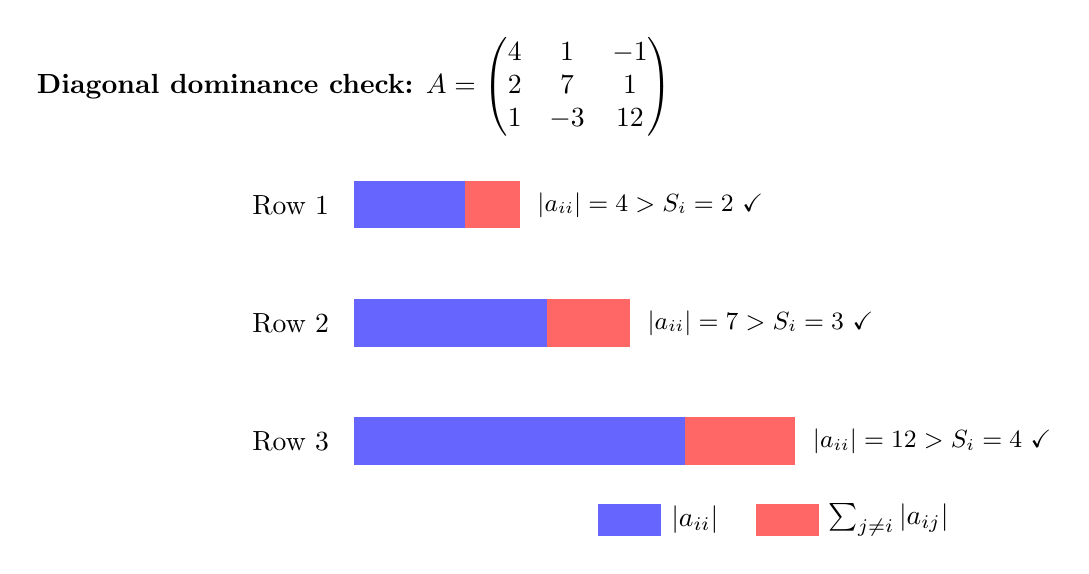
\begin{tikzpicture}
\node at (0,4.5) {\textbf{Diagonal dominance check:} \(A = \begin{pmatrix}4&1&-1\\2&7&1\\1&-3&12\end{pmatrix}\)};
\foreach \row/\diag/\offsum/\ypos in {
  {Row 1}/4/2/3,
  {Row 2}/7/3/1.5,
  {Row 3}/12/4/0}
{
  \node[anchor=east] at (-0.2,\ypos) {\row};
  \fill[blue!60] (0,\ypos-0.3) rectangle (\diag*0.35,\ypos+0.3);
  \fill[red!60] (\diag*0.35,\ypos-0.3) rectangle (\diag*0.35+\offsum*0.35,\ypos+0.3);
  \node[anchor=west] at (\diag*0.35+\offsum*0.35+0.1,\ypos)
    {\small \(|a_{ii}|=\diag > S_i=\offsum\) \checkmark};
}
\node[fill=blue!60, minimum width=0.8cm, minimum height=0.4cm] at (3.5,-1) {};
\node[anchor=west] at (3.9,-1) {\(|a_{ii}|\)};
\node[fill=red!60, minimum width=0.8cm, minimum height=0.4cm] at (5.5,-1) {};
\node[anchor=west] at (5.9,-1) {\(\sum_{j\neq i}|a_{ij}|\)};
\end{tikzpicture}
\end{center}

\subsection*{Visual 4: Error Convergence on Log Scale}

\begin{center}
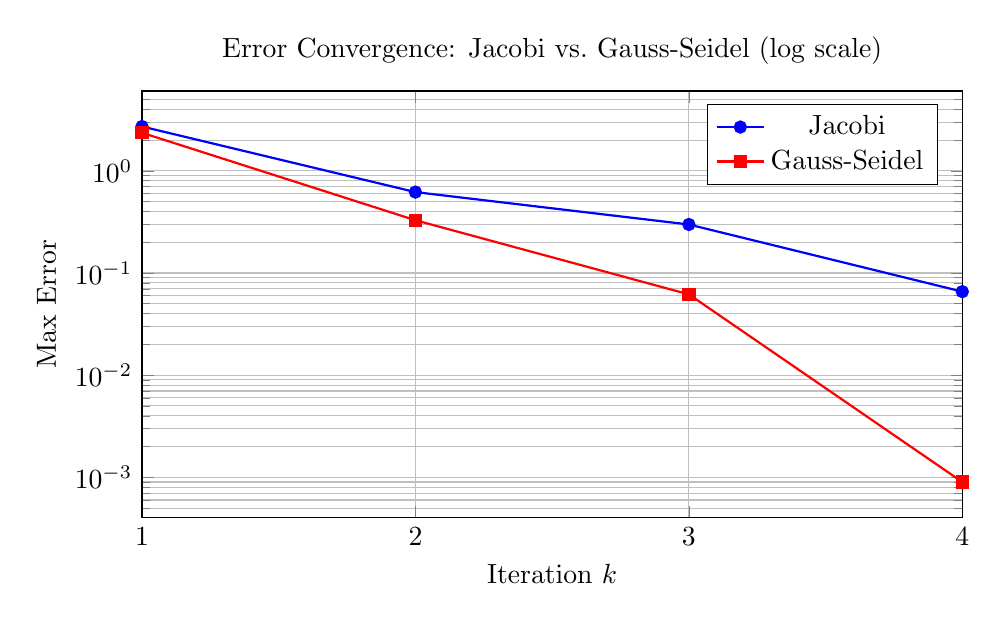
\begin{tikzpicture}
\begin{axis}[
  width=12cm, height=7cm,
  xlabel={Iteration \(k\)},
  ylabel={Max Error},
  title={Error Convergence: Jacobi vs.\ Gauss-Seidel (log scale)},
  ymode=log,
  grid=both,
  legend pos=north east,
  xmin=1, xmax=4,
  xtick={1,2,3,4},
]
\addplot[blue, thick, mark=*] coordinates {
  (1,2.7143)(2,0.6191)(3,0.2983)(4,0.0657)
};
\addlegendentry{Jacobi}
\addplot[red, thick, mark=square*] coordinates {
  (1,2.3571)(2,0.3284)(3,0.0618)(4,0.0009)
};
\addlegendentry{Gauss-Seidel}
\end{axis}
\end{tikzpicture}
\end{center}

%=====================================================================
\section{Step-by-Step Algorithmic Workflows}
%=====================================================================

\textbf{Algorithm 1 --- Pre-Check for Diagonal Dominance}

\begin{enumerate}
  \item Input the \(n \times n\) matrix \(A\) and right-hand side vector \(\mathbf{b}\).
  \item For each row \(i = 1, 2, \ldots, n\):
    \begin{enumerate}[label=\alph*.]
      \item Compute \(D_i = |a_{ii}|\).
      \item Compute \(S_i = \displaystyle\sum_{\substack{j=1\\j\neq i}}^{n}|a_{ij}|\).
      \item If \(D_i \leq S_i\), flag row \(i\) as \emph{not dominant}.
    \end{enumerate}
  \item If all rows pass, declare \(A\) strictly diagonally dominant --- proceed to iterate.
  \item If any row fails: attempt row permutation (swap rows) to place the largest-magnitude
        element on the diagonal for each column. Recheck after rearrangement.
  \item If diagonal dominance cannot be achieved by permutation, use direct methods
        (Gaussian elimination) instead.
\end{enumerate}

\textbf{Algorithm 2 --- Jacobi Method}

\begin{enumerate}
  \item Verify diagonal dominance (Algorithm 1) or confirm \(\rho(B_J) < 1\).
  \item Set initial guess: \(\mathbf{x}^{(0)} = \mathbf{0}\) (or any convenient vector).
  \item Derive the \(n\) Jacobi iteration formulas:
    \[
      x_i^{(k+1)} = \frac{1}{a_{ii}}\!\left[b_i - \sum_{j\neq i}a_{ij}x_j^{(k)}\right],
      \quad i = 1, \ldots, n.
    \]
  \item Compute \(x_1^{(k+1)}, x_2^{(k+1)}, \ldots, x_n^{(k+1)}\)
        using \textbf{only} values from iteration \(k\).
        Store all new values before overwriting the old ones.
  \item Check stopping criterion: \(\max_i|x_i^{(k+1)}-x_i^{(k)}| < \varepsilon\).
  \item If converged, output \(\mathbf{x}^{(k+1)}\) as the solution.
        Otherwise set \(k \leftarrow k+1\) and go to Step 4.
\end{enumerate}

\textbf{Algorithm 3 --- Gauss-Seidel Method}

\begin{enumerate}
  \item Verify diagonal dominance or confirm \(\rho(B_{GS}) < 1\).
  \item Set initial guess: \(\mathbf{x}^{(0)} = \mathbf{0}\).
  \item Derive the \(n\) Gauss-Seidel formulas:
    \[
      x_i^{(k+1)} = \frac{1}{a_{ii}}\!\left[b_i
        - \sum_{j=1}^{i-1}a_{ij}x_j^{(k+1)}
        - \sum_{j=i+1}^{n}a_{ij}x_j^{(k)}\right].
    \]
  \item For \(i = 1\) to \(n\): compute \(x_i^{(k+1)}\) immediately using the
        latest available \(x_j^{(k+1)}\) for \(j < i\) and \(x_j^{(k)}\) for \(j > i\).
        Overwrite \(x_i\) immediately.
  \item Check: \(\max_i|x_i^{(k+1)}-x_i^{(k)}| < \varepsilon\).
  \item If converged, output solution; otherwise \(k \leftarrow k+1\), go to Step 4.
\end{enumerate}

\textbf{Algorithm 4 --- Stopping Criteria Options}

\begin{enumerate}
  \item \textbf{Max absolute change:}
        \(\max_i|x_i^{(k+1)}-x_i^{(k)}| < \varepsilon\) (simplest).
  \item \textbf{Relative change:}
        \(\max_i\dfrac{|x_i^{(k+1)}-x_i^{(k)}|}{|x_i^{(k+1)}|+\delta} < \varepsilon\)
        (avoids issues near zero, \(\delta\) is small).
  \item \textbf{Residual norm:}
        \(\|A\mathbf{x}^{(k+1)}-\mathbf{b}\|_\infty < \varepsilon\)
        (most rigorous; directly measures how well the solution satisfies the equations).
\end{enumerate}

%=====================================================================
\section{Fully Worked Numerical Examples}
%=====================================================================

\subsection*{Example 1 --- Diagonal Dominance Verification}

\textbf{Problem.} Verify that the following system is diagonally dominant and ready
for iterative methods: \(4x_1+x_2-x_3=5\),\quad \(2x_1+7x_2+x_3=19\),\quad
\(x_1-3x_2+12x_3=22\).

\textbf{Solution.}
Matrix of coefficients:
\[
A = \begin{pmatrix} 4 & 1 & -1 \\ 2 & 7 & 1 \\ 1 & -3 & 12 \end{pmatrix}.
\]

Row 1: \(|a_{11}| = 4\). Off-diagonal sum: \(|1| + |-1| = 2\). Check: \(4 > 2\). \textbf{Pass.}

Row 2: \(|a_{22}| = 7\). Off-diagonal sum: \(|2| + |1| = 3\). Check: \(7 > 3\). \textbf{Pass.}

Row 3: \(|a_{33}| = 12\). Off-diagonal sum: \(|1| + |-3| = 4\). Check: \(12 > 4\). \textbf{Pass.}

\textbf{Conclusion:} All three rows satisfy strict diagonal dominance. By the diagonal
dominance theorem, both Jacobi and Gauss-Seidel are guaranteed to converge for this system.

\begin{learnbox}{Key Takeaway}
Always rearrange to achieve diagonal dominance before applying iterative methods.
Attempting to iterate on a non-dominant system is a gamble --- the sequence may diverge
and produce meaningless results.
\end{learnbox}

\subsection*{Example 2 --- Jacobi Method (4 Complete Iterations)}

\textbf{Problem.} Solve the above system by Jacobi's method with
\(\mathbf{x}^{(0)}=(0,0,0)^T\) and tolerance \(\varepsilon=0.05\).

\textbf{Derivation of iteration formulas:}
\[
x_1^{(k+1)} = \frac{1}{4}\!\left[5 - x_2^{(k)} + x_3^{(k)}\right], \quad
x_2^{(k+1)} = \frac{1}{7}\!\left[19 - 2x_1^{(k)} - x_3^{(k)}\right], \quad
x_3^{(k+1)} = \frac{1}{12}\!\left[22 - x_1^{(k)} + 3x_2^{(k)}\right].
\]

All four iterations with complete arithmetic are shown in the table in Section~3 (Jacobi subsection).
The final iterate is \((1.2988, 2.0104, 2.2416)\) with max error \(0.0657 > 0.05\), so
more iterations would be needed for the desired tolerance. The exact solution
\((1.3, 2.0, 2.25)\) shows that Jacobi is converging steadily.

\begin{learnbox}{Key Takeaway}
Jacobi uses ONLY old values --- compute all three updates before using any of them.
This means you need two arrays: one for \(\mathbf{x}^{(k)}\) and one for \(\mathbf{x}^{(k+1)}\).
\end{learnbox}

\subsection*{Example 3 --- Gauss-Seidel (4 Iterations) with Side-by-Side Comparison}

\textbf{Problem.} Solve the same system by Gauss-Seidel with \(\mathbf{x}^{(0)}=(0,0,0)^T\).

All four iterations with complete arithmetic are shown in Section~3 (Gauss-Seidel subsection).
The final iterate after 4 steps is \((1.3020, 2.0236, 2.2307)\) with max error \(0.0009 < 0.05\),
achieving the desired tolerance in 4 iterations. Jacobi required more than 4 iterations for
the same accuracy. The side-by-side comparison table in Section~3 clearly demonstrates
Gauss-Seidel's convergence advantage.

\begin{learnbox}{Key Takeaway}
Gauss-Seidel uses updated values immediately --- converges in roughly half the iterations
of Jacobi. This is the preferred method whenever sequential computation is acceptable.
\end{learnbox}

\subsection*{Example 4 --- Applied: 1D Heat Conduction by Gauss-Seidel}

\textbf{Problem.} A 1D insulated rod has three internal nodes. The steady-state finite
difference equations are:
\[
2T_1 - T_2 = 50, \qquad -T_1 + 2T_2 - T_3 = 0, \qquad -T_2 + 2T_3 = 30.
\]
Apply Gauss-Seidel until the maximum temperature change is less than \(0.01^{\circ}\)C.
Start from \(T_1^{(0)}=T_2^{(0)}=T_3^{(0)}=0\).

\textbf{Check diagonal dominance:}
Row 1: \(|2|=2 > |-1|=1\). Row 2: \(|2|=2 > |-1|+|-1|=2\). Row 2 satisfies
\(|a_{22}|=2\) and \(\sum_{j\neq 2}|a_{2j}|=2\), which is NOT strict dominance
(\(2 \not> 2\)). However, for symmetric positive definite tridiagonal matrices of this
form, Gauss-Seidel is known to converge regardless. Row 3: \(|2|=2 > 1\). We proceed.

\textbf{Gauss-Seidel formulas:}
\[
T_1^{(k+1)} = \frac{1}{2}\!\left[50 + T_2^{(k)}\right], \quad
T_2^{(k+1)} = \frac{1}{2}\!\left[T_1^{(k+1)} + T_3^{(k)}\right], \quad
T_3^{(k+1)} = \frac{1}{2}\!\left[30 + T_2^{(k+1)}\right].
\]

\textbf{Iteration 1} (from \((0,0,0)\)):
\begin{align*}
T_1^{(1)} &= \tfrac{1}{2}[50 + 0] = 25.0000 \\
T_2^{(1)} &= \tfrac{1}{2}[25.0000 + 0] = 12.5000 \\
T_3^{(1)} &= \tfrac{1}{2}[30 + 12.5000] = 21.2500
\end{align*}
Max change \(= 25.0000\).

\textbf{Iteration 2}:
\begin{align*}
T_1^{(2)} &= \tfrac{1}{2}[50 + 12.5000] = 31.2500 \\
T_2^{(2)} &= \tfrac{1}{2}[31.2500 + 21.2500] = 26.2500 \\
T_3^{(2)} &= \tfrac{1}{2}[30 + 26.2500] = 28.1250
\end{align*}
Max change \(= \max(6.2500, 13.7500, 6.8750) = 13.7500\).

\textbf{Iteration 3}:
\begin{align*}
T_1^{(3)} &= \tfrac{1}{2}[50 + 26.2500] = 38.1250 \\
T_2^{(3)} &= \tfrac{1}{2}[38.1250 + 28.1250] = 33.1250 \\
T_3^{(3)} &= \tfrac{1}{2}[30 + 33.1250] = 31.5625
\end{align*}
Max change \(= \max(6.8750, 6.8750, 3.4375) = 6.8750\).

\textbf{Iteration 4}:
\begin{align*}
T_1^{(4)} &= \tfrac{1}{2}[50 + 33.1250] = 41.5625 \\
T_2^{(4)} &= \tfrac{1}{2}[41.5625 + 31.5625] = 36.5625 \\
T_3^{(4)} &= \tfrac{1}{2}[30 + 36.5625] = 33.2813
\end{align*}
Max change \(= \max(3.4375, 3.4375, 1.7188) = 3.4375\).

Continuing this process, after approximately 15 iterations the solution converges to
\(T_1 \approx 47.5^{\circ}\)C, \(T_2 \approx 45.0^{\circ}\)C, \(T_3 \approx 37.5^{\circ}\)C
(the exact solution found by solving the tridiagonal system directly).

\textbf{Physical interpretation:} Node 1 is closest to the hot boundary (left BC gives
\(T_0\) implicitly at \(50^{\circ}\)C effective), Node 3 is closest to the cooler right
boundary. The temperature gradient from Node 1 to Node 3 represents heat flowing left to right.

\begin{learnbox}{Key Takeaway}
Iterative methods naturally suit FD/FEA problems where the matrix is large, sparse, and
diagonally dominant (or symmetric positive definite). In a typical 2D heat conduction
problem with \(100 \times 100\) nodes, the system is \(10000 \times 10000\) --- Gauss-Seidel
solves it efficiently; Gaussian elimination would require storing \(10^8\) entries.
\end{learnbox}

%=====================================================================
\section{Tabular Reference and Comparison}
%=====================================================================

\subsection*{Method Feature Comparison}

\begin{center}
\begin{tabular}{@{}p{3.5cm}p{4.5cm}p{4.5cm}@{}}
\toprule
\textbf{Feature} & \textbf{Jacobi} & \textbf{Gauss-Seidel} \\
\midrule
Update rule &
  All \(x_i^{(k+1)}\) computed from \(\mathbf{x}^{(k)}\) only &
  \(x_i^{(k+1)}\) uses freshest available values \\
\addlinespace
Iteration matrix &
  \(B_J = D^{-1}(L+U)\) &
  \(B_{GS} = (D+L)^{-1}U\) \\
\addlinespace
Memory &
  Needs two arrays (\(\mathbf{x}^{(k)}\) and \(\mathbf{x}^{(k+1)}\)) &
  Can overwrite in place (one array) \\
\addlinespace
Parallelism &
  Fully parallelisable (all updates independent) &
  Sequential (each update depends on previous) \\
\addlinespace
Convergence speed &
  Slower; \(\rho(B_J)\) often larger &
  \(\approx 2\times\) faster; \(\rho(B_{GS})\approx\rho(B_J)^2\) \\
\addlinespace
Convergence condition &
  Diagonal dominance or \(\rho(B_J)<1\) &
  Same; also converges for SPD matrices \\
\addlinespace
Typical application &
  Parallel computing architectures (GPU) &
  General serial computation; power systems \\
\addlinespace
Programming effort &
  Slightly more (two arrays required) &
  Simpler (in-place update) \\
\bottomrule
\end{tabular}
\end{center}

\subsection*{Iteration Summary Table Template}

Students may use this template to record iterations during practice:

\begin{center}
\begin{tabular}{@{}ccccc@{}}
\toprule
Iteration \(k\) & \(x_1^{(k)}\) & \(x_2^{(k)}\) & \(x_3^{(k)}\) & Max Error \\
\midrule
0 & & & & --- \\
1 & & & & \\
2 & & & & \\
3 & & & & \\
4 & & & & \\
\ldots & & & & \\
Exact & & & & 0 \\
\bottomrule
\end{tabular}
\end{center}

%=====================================================================
\section{Common Student Mistakes}
%=====================================================================

\begin{mistakebox}{Common Errors in Applying Iterative Methods --- Study and Avoid}
\begin{tabular}{@{}p{4cm}p{5cm}p{4.5cm}@{}}
\toprule
\textbf{Mistake} & \textbf{What Goes Wrong} & \textbf{Correct Practice} \\
\midrule
Using updated \(x\) values inside the Jacobi step &
  Accidentally mixing Jacobi and Gauss-Seidel; results are neither method
  and may not converge at the theoretically predicted rate &
  In Jacobi, always freeze all \(x^{(k)}\) values at the start of iteration \(k\);
  use only the frozen values throughout \\
\addlinespace
Skipping the diagonal dominance check &
  Iteration may diverge silently; the computed sequence grows without bound
  or oscillates &
  Always check \(|a_{ii}| > \sum_{j\neq i}|a_{ij}|\) for every row
  before starting iterations \\
\addlinespace
Checking only one variable for convergence &
  Stopping too early because one variable has converged while others have not;
  solution is inaccurate &
  Always compute max error over \emph{all} variables:
  \(\max_i|x_i^{(k+1)}-x_i^{(k)}|\) \\
\addlinespace
Failing to rearrange to dominant form &
  Applying iteration to a non-dominant system and wondering why it diverges;
  the row permutation needed is trivial &
  Identify the largest entry in each column and move it to the diagonal
  by swapping rows before proceeding \\
\addlinespace
Stopping at the wrong iteration &
  Either stopping too early (tolerance not met, inaccurate answer) or
  iterating unnecessarily long (wasted computation) &
  Use the stopping criterion \(\max_i|x_i^{(k+1)}-x_i^{(k)}| < \varepsilon\)
  after every step; set \(\varepsilon\) to match the required decimal accuracy \\
\bottomrule
\end{tabular}
\end{mistakebox}

%=====================================================================
\section{Assessment Suite}
%=====================================================================

\subsection*{Viva-Voce Questions}

\begin{enumerate}
  \item What is a strictly diagonally dominant matrix? Write the row-wise condition mathematically.
  \item State the convergence theorem for diagonally dominant matrices as applied to iterative methods.
  \item How do you check whether a \(3 \times 3\) matrix is diagonally dominant? If it is not,
        what is the standard remedial action?
  \item In the Jacobi method, why must you compute ALL updated values before overwriting the old ones?
        What error occurs if you update in place?
  \item Write the Jacobi iteration formula for the \(i\)-th variable in a general \(n \times n\) system.
  \item Write the matrix form of the Jacobi iteration, identifying \(D\), \(L\), and \(U\).
  \item In the Gauss-Seidel method, explain what ``sequential update'' means using the formulas
        for \(x_1^{(k+1)}\), \(x_2^{(k+1)}\), and \(x_3^{(k+1)}\).
  \item Why does Gauss-Seidel typically converge faster than Jacobi? State the exact relationship
        between their spectral radii for tridiagonal systems.
\end{enumerate}

\subsection*{Descriptive Problems}

\begin{enumerate}
  \item Solve the system \(5x_1 - x_2 + x_3 = 10\), \(2x_1 + 8x_2 - x_3 = 11\),
        \(x_1 + x_2 + 4x_3 = 12\) by the Jacobi method. Perform 5 iterations starting from
        \(\mathbf{x}^{(0)} = (0,0,0)^T\). Present results in a full iteration table and
        compare with the exact solution.
  \item Apply Gauss-Seidel to the system in Problem 1. Perform iterations until
        \(\max_i|x_i^{(k+1)}-x_i^{(k)}| < 0.005\). Show complete arithmetic for each iteration.
        How many iterations were required compared to Jacobi?
  \item A structural FEA problem yields the system \(6u_1 - u_2 = 5\), \(-u_1 + 6u_2 - u_3 = 0\),
        \(-u_2 + 6u_3 = 5\) (all in mm). Verify diagonal dominance, compute \(\rho(B_J)\) and
        \(\rho(B_{GS})\), and apply Gauss-Seidel for 4 iterations.
  \item For the matrix \(A = \begin{pmatrix}3&1\\1&3\end{pmatrix}\), compute \(B_J\) and
        \(B_{GS}\) explicitly. Find \(\rho(B_J)\) and \(\rho(B_{GS})\). Verify that
        \(\rho(B_{GS}) = \rho(B_J)^2\).
\end{enumerate}

\subsection*{Multiple Choice Questions}

\begin{enumerate}

\item A matrix \(A\) is strictly diagonally dominant if, for every row \(i\):
\begin{enumerate}[label=\Alph*.]
  \item \(|a_{ii}| = \displaystyle\sum_{j\neq i}|a_{ij}|\)
  \item \(|a_{ii}| < \displaystyle\sum_{j\neq i}|a_{ij}|\)
  \item \(\textbf{|a}_{ii}\textbf{|} > \displaystyle\sum_{j\neq i}\textbf{|a}_{ij}\textbf{|}\)
  \item \(|a_{ii}| \geq \displaystyle\sum_{j\neq i}|a_{ij}|\)
\end{enumerate}
\textit{Answer: C.} Strict inequality \(|a_{ii}| > \sum_{j\neq i}|a_{ij}|\) is required
for every row --- equality is not sufficient for the strict dominance convergence guarantee.

\item In the Jacobi method, the value \(x_i^{(k+1)}\) is computed using:
\begin{enumerate}[label=\Alph*.]
  \item The latest computed values of all \(x_j^{(k+1)}\)
  \item \(\textbf{All values from the previous iteration }x_j^{(k)}\textbf{ only}\)
  \item A mix of old and new values depending on convergence
  \item Values from two iterations back, \(x_j^{(k-1)}\)
\end{enumerate}
\textit{Answer: B.} This is the defining property of Jacobi: all updates use only the frozen
previous-iteration values, enabling parallel computation.

\item Which of the following is the correct Jacobi iteration matrix for \(A = D + L + U\)?
\begin{enumerate}[label=\Alph*.]
  \item \(B_J = (D+L)^{-1}U\)
  \item \(B_J = D^{-1}(L+U)\)
  \item \(\textbf{B}_J = \mathbf{-D}^{-1}\mathbf{(L+U)}\)
  \item \(B_J = -(D+L)^{-1}U\)
\end{enumerate}
\textit{Answer: C.} The Jacobi iteration is \(\mathbf{x}^{(k+1)} = -D^{-1}(L+U)\mathbf{x}^{(k)}
+ D^{-1}\mathbf{b}\), so \(B_J = -D^{-1}(L+U)\).

\item The iterative method converges for any starting point if and only if:
\begin{enumerate}[label=\Alph*.]
  \item The matrix \(A\) is symmetric
  \item The determinant of \(A\) is positive
  \item The trace of the iteration matrix is less than 1
  \item \(\textbf{The spectral radius } \rho(B) < 1\)
\end{enumerate}
\textit{Answer: D.} The spectral radius condition \(\rho(B) < 1\) is the necessary and
sufficient condition for convergence of any stationary linear iterative method.

\item For a consistently ordered tridiagonal matrix, the relationship between the spectral
radii of Jacobi and Gauss-Seidel is:
\begin{enumerate}[label=\Alph*.]
  \item \(\rho(B_{GS}) = \rho(B_J) / 2\)
  \item \(\rho(B_{GS}) = 2\rho(B_J)\)
  \item \(\rho(B_{GS}) = \rho(B_J)\)
  \item \(\boldsymbol{\rho(B_{GS}) = [\rho(B_J)]^2}\)
\end{enumerate}
\textit{Answer: D.} For consistently ordered matrices, \(\rho(B_{GS}) = \rho(B_J)^2\),
which explains why Gauss-Seidel needs approximately half as many iterations.

\item In the Gauss-Seidel method, when computing \(x_3^{(k+1)}\) in a \(3 \times 3\) system,
the formula uses:
\begin{enumerate}[label=\Alph*.]
  \item \(x_1^{(k)}\) and \(x_2^{(k)}\) (all old)
  \item \(x_1^{(k+1)}\) (new) and \(x_2^{(k)}\) (old)
  \item \(\textbf{x}_1^{(k+1)}\) \textbf{and} \(\mathbf{x}_2^{(k+1)}\) \textbf{(both new)}
  \item \(x_1^{(k)}\) (old) and \(x_2^{(k+1)}\) (new)
\end{enumerate}
\textit{Answer: C.} Since \(i=3 > j=1\) and \(i=3 > j=2\), both \(x_1\) and \(x_2\)
have already been updated in the current iteration and are used in their newest form.

\end{enumerate}

%=====================================================================
\section{Quick Recap and Formula Sheet}
%=====================================================================

\begin{learnbox}{Formula Sheet: Iterative Methods for Linear Systems}
\begin{itemize}
  \item \textbf{Diagonal dominance:} \(|a_{ii}| > \displaystyle\sum_{j\neq i}|a_{ij}|\)
        for all rows --- sufficient condition for both Jacobi and Gauss-Seidel convergence.
  \item \textbf{Jacobi update:} \(x_i^{(k+1)} = \dfrac{1}{a_{ii}}\!\left[b_i -
        \displaystyle\sum_{j\neq i}a_{ij}x_j^{(k)}\right]\) --- uses ONLY old values \(x^{(k)}\).
  \item \textbf{Gauss-Seidel update:} \(x_i^{(k+1)} = \dfrac{1}{a_{ii}}\!\left[b_i
        - \displaystyle\sum_{j<i}a_{ij}x_j^{(k+1)} - \displaystyle\sum_{j>i}a_{ij}x_j^{(k)}
        \right]\) --- uses updated values \(x_j^{(k+1)}\) for \(j < i\) immediately.
  \item \textbf{GS convergence advantage:} Gauss-Seidel converges in approximately \(2\times\)
        fewer iterations than Jacobi for the same system.
  \item \textbf{Stopping criterion:} \(\max_i\left|x_i^{(k+1)} - x_i^{(k)}\right| < \varepsilon\)
        --- check over ALL variables after each full iteration.
  \item \textbf{Initial guess:} \(\mathbf{x}^{(0)} = \mathbf{0}\) (zero vector) is the
        standard starting point when no better guess is available.
  \item \textbf{Matrix splitting:} Jacobi uses \(M=D\); Gauss-Seidel uses \(M=(D+L)\).
        Convergence iff spectral radius \(\rho(M^{-1}N) < 1\).
  \item \textbf{Best suited for:} Large, sparse, diagonally dominant systems arising in
        FEM, FDM, power systems, and network analysis --- where direct methods are too costly.
\end{itemize}
\end{learnbox}

\end{document}
